\documentclass[12pt]{article}

%%%%%%%%%%%%%%%%%%%
% Packages/Macros %
%%%%%%%%%%%%%%%%%%%
\usepackage{amssymb,latexsym,amsmath}     % Standard packages
\usepackage{graphicx}
\usepackage{subcaption}
%\usepackage{subfig}
%\usepackage[caption=false]{subfig}
\usepackage{cite} % Allows for ranges in citation
\usepackage{mciteplus}
\usepackage[toc,page]{appendix}
\usepackage{titlesec}
\usepackage{xcolor}
\usepackage{hyperref}    % Hyperlinks in references
%\usepackage[all]{hypcap} % Internal hyperlinks to floats.
\definecolor{darkblue}{rgb}{0,0,0}
\definecolor{darkgreen}{rgb}{0,0.5,0}
\definecolor{darkviolet}{rgb}{0.55,0.,0.55}
\hypersetup{colorlinks=true, linkcolor=darkblue, citecolor=darkviolet, urlcolor=darkgray}
%\usepackage{array}
\usepackage{booktabs}
\usepackage[inner=2.9cm,outer=2.6cm,bottom=2.6cm]{geometry}
%%%%%%%%%%%
% Margins % 
%%%%%%%%%%%
%\addtolength{\textwidth}{2.3in}
%\addtolength{\textheight}{2.3in}
%\addtolength{\evensidemargin}{-1.2in}
%\addtolength{\oddsidemargin}{-1.2in}
%\addtolength{\topmargin}{-1.2in}
%\usepackage[usenames,dvipsnames,svgnames,table]{xcolor}

%%%%%%%%%%%%%%%%%%%%%%%%%%%%%%
% Theorem/Proof Environments %
%%%%%%%%%%%%%%%%%%%%%%%%%%%%%%
\newtheorem{theorem}{Theorem}
\newenvironment{proof}{\noindent{\bf Proof:}}{$\hfill \Box$ \vspace{10pt}}  


%% THis file contains all the default packages and modifications for
% LHCb formatting

%% %%%%%%%%%%%%%%%%%%
%%  Page formatting
%% %%%%%%%%%%%%%%%%%%
\usepackage[inner=2.9cm,outer=2.6cm,bottom=2.6cm]{geometry}

\raggedbottom
% To avoid Latex to be too fussy with line breaking ...
\sloppy

%%% Header
\usepackage{fancyhdr}
\pagestyle{fancy}
\fancyhead[RO,LE]{}
\fancyhead[LO]{\itshape \nouppercase\leftmark}
\fancyhead[RE]{\itshape \nouppercase\rightmark}
\setlength{\headheight}{15pt}


%%At the beginning of chapter make half page free space
%\usepackage{setspace}
%\onehalfspacing

%% %%%%%%%%%%%%%%%%%%%%%%%
%% Packages to be used
%% %%%%%%%%%%%%%%%%%%%%%%%
\usepackage{microtype}
\usepackage{lineno}  % for line numbering during review
\usepackage{xspace} % To avoid problems with missing or double spaces after
\usepackage{ulem}
%\usepackage{hepnames}

%% Graphics
\usepackage{graphicx}  % to include figures (can also use other packages)
\usepackage{color}
\usepackage{xcolor}
\usepackage{colortbl}
\usepackage{rotating}
\usepackage{subfigure}
\usepackage{epstopdf}
\graphicspath{{./figs/}} % Make Latex search fig subdir for figures

%%Tables
\usepackage{longtable} % only for template; not usually to be used in PAPERs
\usepackage{multirow}


%% Math
\usepackage{amssymb,amsfonts,amsmath,mathtext}
\usepackage{amsmath} % Adds a large collection of math symbols
\usepackage{amssymb}
\usepackage{amsfonts}
\usepackage{upgreek} % Adds in support for greek letters in roman typeset
\usepackage{breqn} %%two lines in formulas

%%Diagamms
\usepackage{tikz}
\usetikzlibrary{decorations.pathreplacing,decorations.pathmorphing,decorations.markings,trees,calc,patterns,decorations}

%% fix to allow peaceful coexistence of line numbering and
%% mathematical objects
%% http://www.latex-community.org/forum/viewtopic.php?f=5&t=163
%%
\newcommand*\patchAmsMathEnvironmentForLineno[1]{%
\expandafter\let\csname old#1\expandafter\endcsname\csname #1\endcsname
\expandafter\let\csname oldend#1\expandafter\endcsname\csname
end#1\endcsname
 \renewenvironment{#1}%
   {\linenomath\csname old#1\endcsname}%
   {\csname oldend#1\endcsname\endlinenomath}%
}
\newcommand*\patchBothAmsMathEnvironmentsForLineno[1]{%
  \patchAmsMathEnvironmentForLineno{#1}%
  \patchAmsMathEnvironmentForLineno{#1*}%
}
\AtBeginDocument{%
\patchBothAmsMathEnvironmentsForLineno{equation}%
\patchBothAmsMathEnvironmentsForLineno{align}%
\patchBothAmsMathEnvironmentsForLineno{flalign}%
\patchBothAmsMathEnvironmentsForLineno{alignat}%
\patchBothAmsMathEnvironmentsForLineno{gather}%
\patchBothAmsMathEnvironmentsForLineno{multline}%
}

% Get hyperlinks to captions and in references.
% These do not work with revtex. Use "hypertext" as class option instead.
\usepackage{hyperref}    % Hyperlinks in references
%\usepackage[all]{hypcap} % Internal hyperlinks to floats.
\definecolor{darkblue}{rgb}{0,0,0.5}
\definecolor{darkgreen}{rgb}{0,0.5,0}
\definecolor{darkviolet}{rgb}{0.55,0.,0.55}
\hypersetup{colorlinks=true, linkcolor=darkblue, citecolor=darkviolet, urlcolor=darkgray}
%\usepackage[all]{hypcap} % Internal =hyperlinks to floats.

\input{lhcb-symbols-def} % Add in the predefined LHCb symbols

% Make this the last packages you include before the \begin{document}
%%%\usepackage{citesort} % automatically sort citations
\usepackage{bibentry} 
\usepackage{cite} % Allows for ranges in citations
\usepackage{mciteplus}

\usepackage{array}
\newcolumntype{L}[1]{>{\raggedright\let\newline\\\arraybackslash\hspace{0pt}}m{#1}}
\newcolumntype{C}[1]{>{\centering\let\newline\\\arraybackslash\hspace{0pt}}m{#1}}
\newcolumntype{R}[1]{>{\raggedleft\let\newline\\\arraybackslash\hspace{0pt}}m{#1}}

\usepackage{titlesec}
%%%%%%%%%%%%
% Document %
%%%%%%%%%%%%
\begin{document}

%%%%%%%%%%%%%%%%%%%%%%%%%
%%%%%  TITLE PAGE  %%%%%%
%%%%%%%%%%%%%%%%%%%%%%%%%
\begin{titlepage}
\begingroup
    \fontsize{14pt}{12pt}\selectfont
    

% Header ---------------------------------------------------
\vspace*{-1.5cm}


%\vspace*{1.0cm}

% Authors -------------------------------------------------

%\begin{center} 
%\bf UNIVERSIT\'{E} PARIS-SUD XI \\
%\end{center}
%\begin{center} 
%\vspace*{0.5cm}
%\'{E}cole Doctorale : Particules, Noyaux et Cosmos - ED 517 \\
%Laboratoire de l'Acc\'{e}l\'{e}rateur Lin\'{e}aire - UMR 8607 \\
%{\it\small
%Centre Scientifique d'Orsay, B\^{a}timent 200 - BP 34, 91898 Orsay CEDEX - France 
%}
%\end{center}

%\begin{center}
%\vspace*{0.5cm}
%Discipline : Physique des particules
%\end{center}

\vspace*{1cm}
%\begin{center}
%\bf 
%TH\'{E}SE DE DOCTORAT\\
%\end{center}

%\begin{center}
%{\normalsize
%pr\'{e}sent\'{e}e par\\
%}
%\end{center}
%\vspace*{-0.5cm}
%\begin{center}
%Olga KOCHEBINA
%\end{center}

% Title --------------------------------------------------

\begin{center}

\includegraphics[width=.5\textwidth]{figs/root_logo.png}
\end{center}

\vspace*{1cm}
{\boldmath\huge
\begin{center}
\textbf{ROOT manual for GATE users}
\end{center}
}

\vspace*{1cm}
\begin{center}
Olga KOCHEBINA
\end{center}
\begin{center}
kochebina@gmail.com
\end{center}

\begin{center}
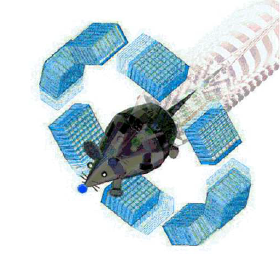
\includegraphics[width=.5\textwidth]{figs/gate_logo.png}
\end{center}

\vspace*{1cm}
\begin{center}
Version 1.0\\
\vspace*{0.5cm}
\today
\end{center}
%\end{tabular*}

\vspace*{5.0cm}
%\begin{center}
%{\normalsize
%Soutenue le 19 Septembre 2014 devant le Jury compos\'{e} de :\\

%\begin{tabular}{lll}
%Mme. & Vera LUTH & Rapporteur\\
%M. & Urs LANGENEGGER & Examinateur\\
%Mme. & Svjetlana FAJFER & Examinateur\\
%M. & Guy WILKINSON & Rapporteur \\
%M. & Achille STOCCHI & Pr\'{e}sident \\
%Mme. & Marie-H\'{e}l\`{e}ne SCHUNE   & Directrice de th\'{e}se \\
%M. & Benoit VIAUD & Examinateur\\
%\end{tabular}
%}
%\end{center}
\vspace{\fill}



\vspace*{1.5cm}
\vspace{\fill}
\endgroup
\end{titlepage}


\pagestyle{empty}  % no page number for the title 

%%%%%%%%%%%%%%%%%%%%%%%%%%%%%%%%
%%%%%  EOD OF TITLE PAGE  %%%%%%
%%%%%%%%%%%%%%%%%%%%%%%%%%%%%%%%

%  empty page follows the title page ----
\newpage
\setcounter{page}{2}



\title{ROOT manual for GATE users}
%\author{Olga Kochebina}
%\maketitle
\tableofcontents
\newpage
\begin{abstract}
The manual for GATE users who wants to become a friend with ROOT output files. This documents contains the simplest actions with a ROOT files. They are so simple that you cannot find it easily. In some sense it is the manual of "From what to begin" of ROOT using.  Please, don't hesitate to contact \textcolor{blue}{kochebina@gmail.com} if you have any questions and comments. And of course, I strongly invite you to visit and use the ROOT web site, \href{https://root.cern.ch/}{https://root.cern.ch/}. This manual is very brief introduction and may just help you only in your first steps. Anyway, I hope that this document will save you some time.
\begin{center}
Have fun!
\end{center}
 

\vspace*{10cm}

\textit{I'd like to thank Benoit VIAUD who thought me almost everything that you will find in this manual.}   
\end{abstract}



\pagebreak


%%%%%%%%%%%%%%%%%%%%%%%%%%%%%%%%%%%%%%%%%%%%%%%%%%%
\section{Obtain your ROOT file}
The standard way to get ROOT out put is to add in your macro:
\\
\verb|/gate/output/root/enable | \\
\verb|/gate/output/root/setFileName        YourOutputFile|
\\
This command creates a file \verb| YourOutputFile.root|, which contains usually several ROOT TTree objects, like Hits, Singles, Coincidences. TTree is .... 

\

One can choose the standard TTree with commands:\\
\verb|/gate/output/root/setRootHitFlag         1| \\
\verb|/gate/output/root/setRootSinglesFlag      1|

It is possible to have some additional TTrees, for example, with an energy selection. To do so one should add in digitizer something like: \\
\verb|/gate/digitizer/name peak171| \\
\verb|/gate/digitizer/insert singleChain| \\
\verb|/gate/digitizer/peak171/setInputName Singles| \\
\verb|/gate/digitizer/peak171/insert thresholder| \\
\verb|/gate/digitizer/peak171/thresholder/setThreshold 153.9 keV| \\
\verb|/gate/digitizer/peak171/insert upholder| \\
\verb|/gate/digitizer/peak171/upholder/setUphold 188.1 keV| \\
This will add to the .root file a TTree with a name peak171 which will contain Singles events with energies [153.9,188.1]~keV.
 

\section{Painless ROOT file opening}
The simplest way to open your ROOT file is to type in terminal:\\
\verb|> root -l YourOutputFile.root |\\
option -l will remove the ROOT start image. 

There are two ways to check the content of your file:
\begin{enumerate}
\item use a \verb|TBrowser|, which is not very powerful and gives an access to visualized structure of your ROOT file but very limited if for selection application or two histograms superposition
\item I \textbf{strongly recommend} use command:\\

root[0]\verb| .ls|\\

This command will show you the list of all ROOT objects that you have in your file or that you created in the current ROOT session (see Figure~\ref{fig:.ls}). The names of TTree's are often repeated twice, this should not bother you. 
\end{enumerate}
\begin{figure}[h]
\centering
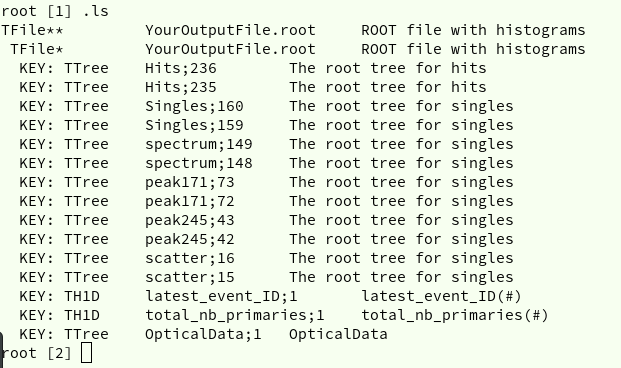
\includegraphics[scale=0.5]{figs/ls.png}
\caption{Output of .ls command}
\label{fig:.ls}
\end{figure}
\clearpage
In order to get the content of each TTree, i.e. list of saved histograms
or "branches", for example for Hits TTree, one should do:\\

root[1] \verb| Hits->Show()| \\

The results of this command is shown in Figure~\ref{fig:Show}

\begin{figure}[h]
\centering
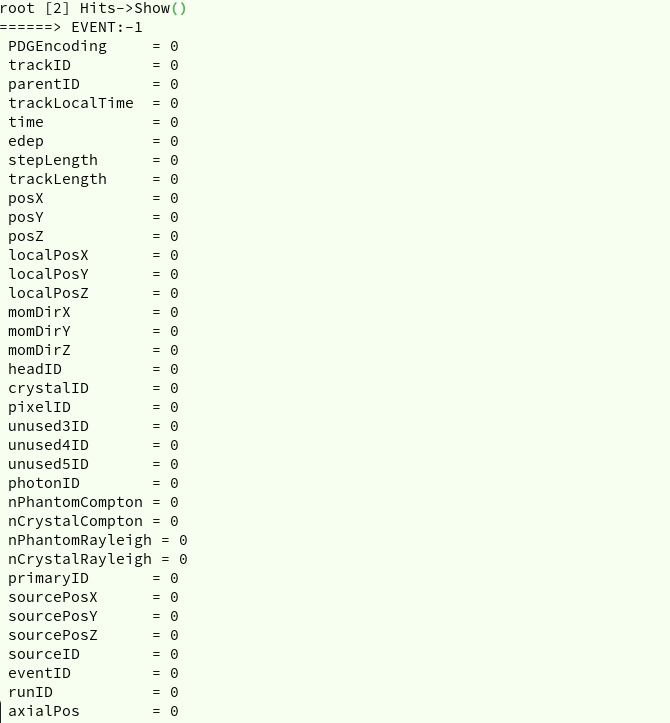
\includegraphics[scale=0.5]{figs/Show.png}
\caption{Output of Show() command}
\label{fig:Show}
\end{figure}



\section{Smart plotting of your histograms (without TBrowser and python scripts)}
To plot a histogram one should use option \verb|TTree -> Draw("name_of_the_branch")|. For example, if you want to plot 1D, 2D or 3D histograms of energy you could do    

root[1] \verb| Hits->Draw("edep")| for 1D (Figure~\ref{fig:1Dhist}, top) \\

root[2] \verb| Hits->Draw("posX:posY")| for 2D, where the first argument, \verb|posX| is ordinate axis and \verb|posY| is abscissa axis  (Figure~\ref{fig:1Dhist}, middle)\\

root[3] \verb| Hits->Draw("posX:posY:posZ")| for 3D (Figure~\ref{fig:1Dhist}, bottom)\\
\begin{figure}[h]
\centering
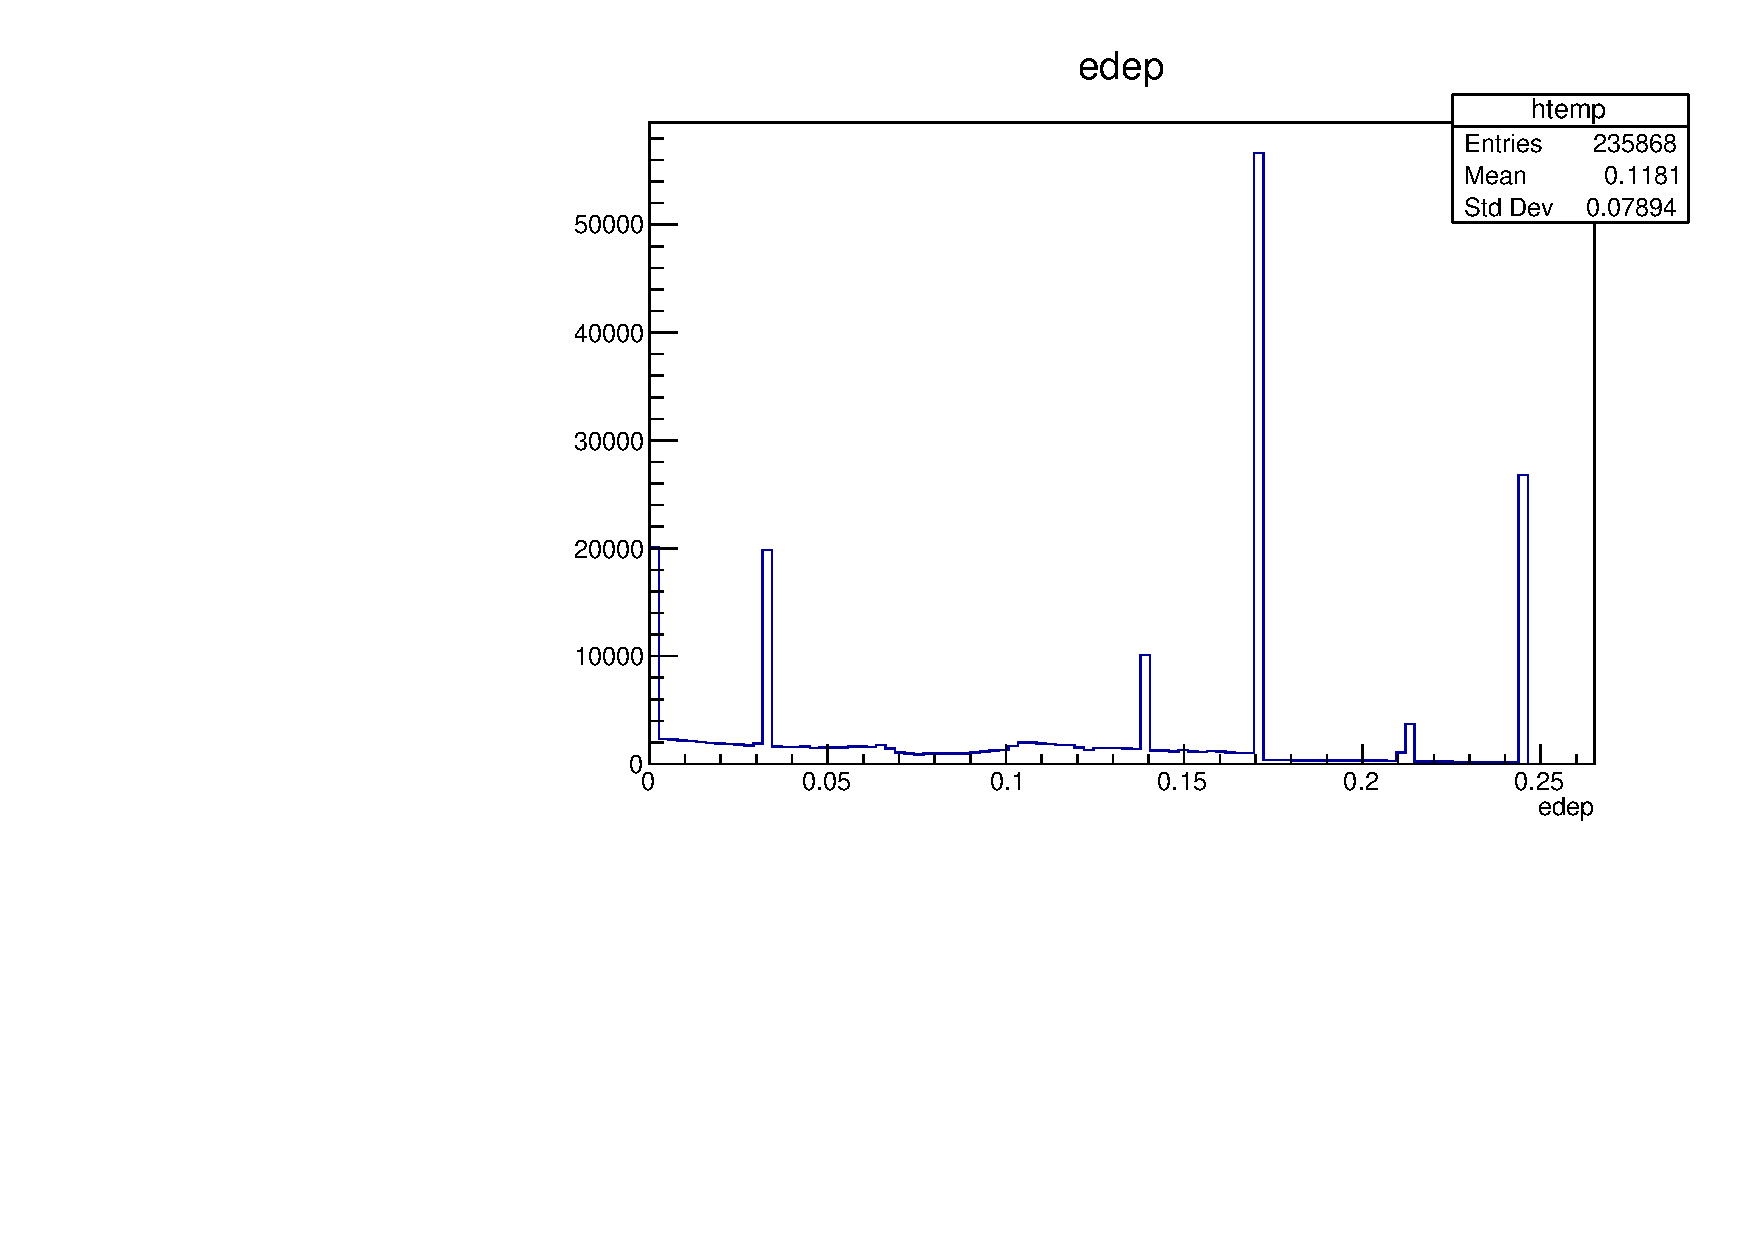
\includegraphics[scale=0.37]{figs/1Dhist.pdf} \\
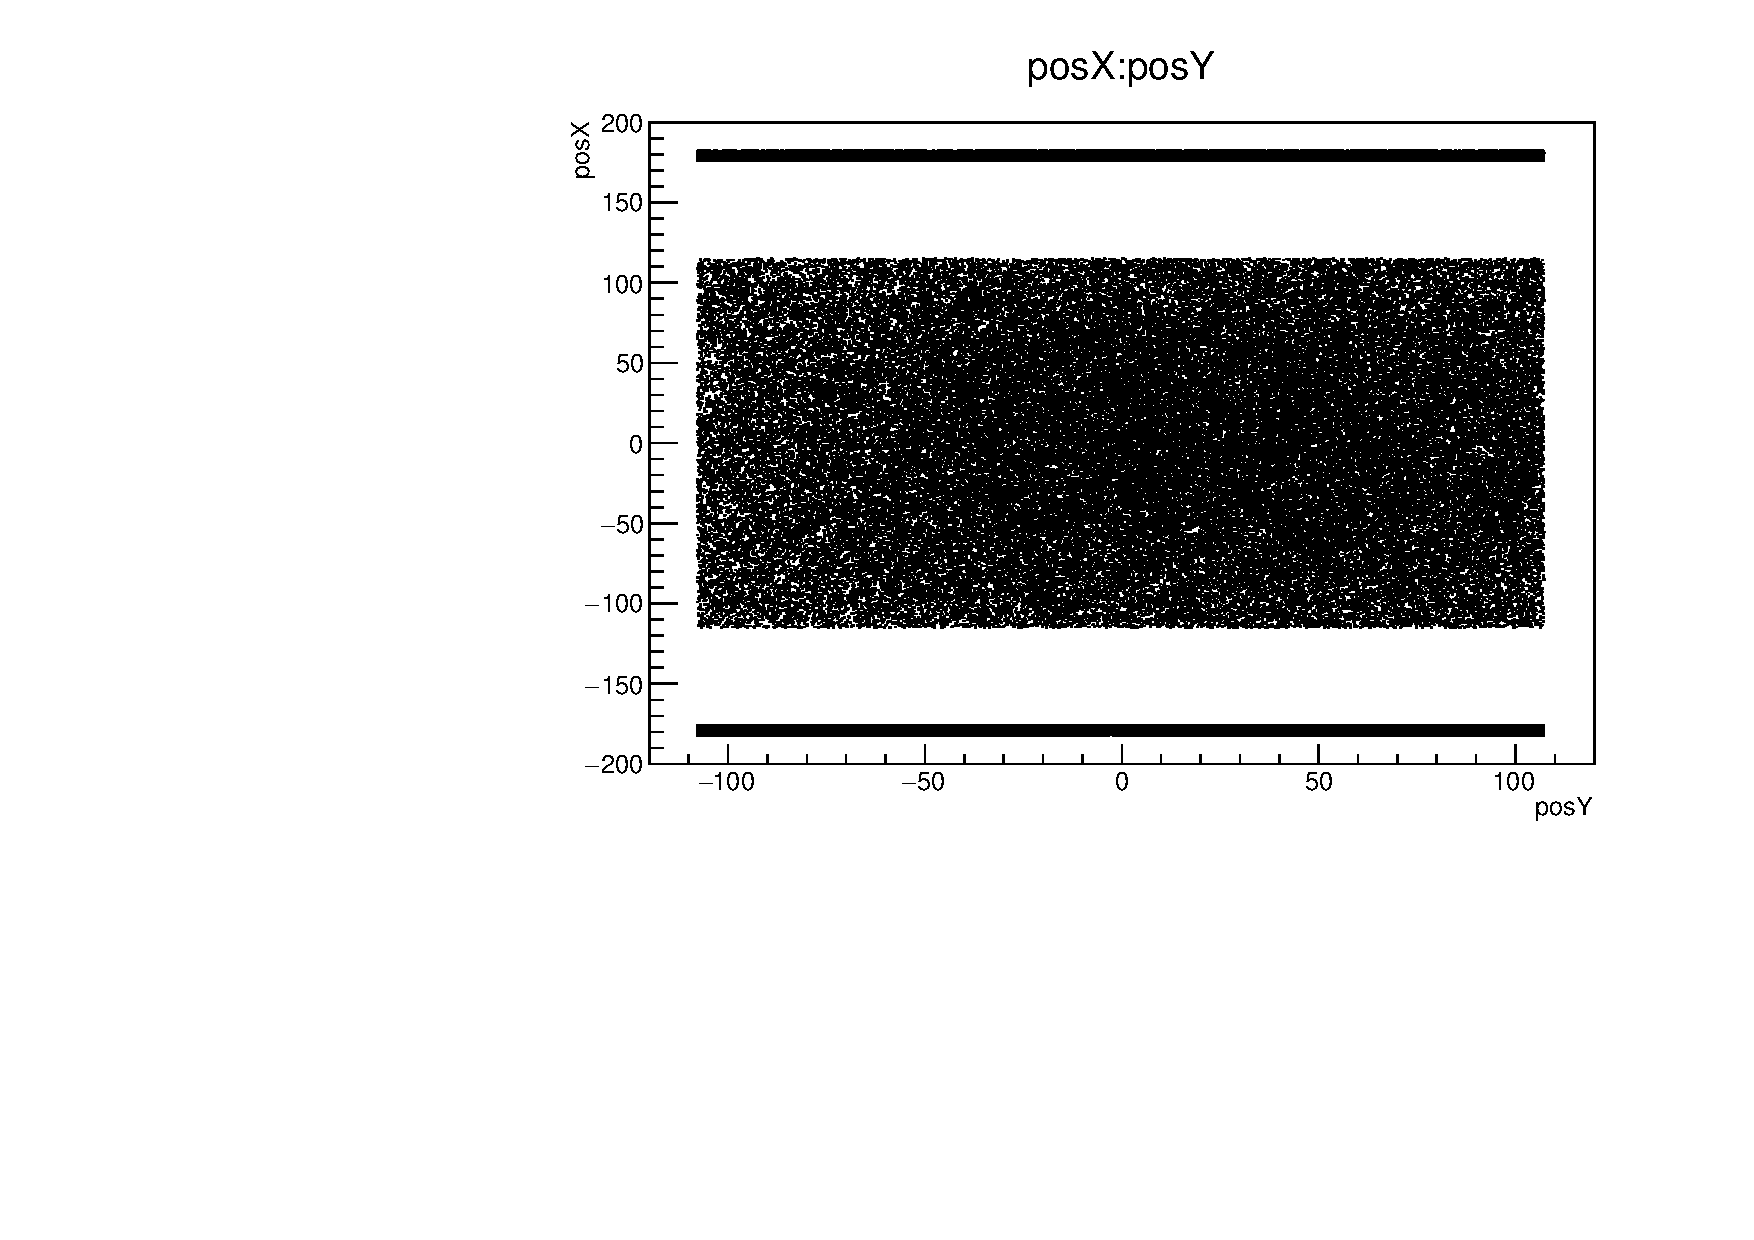
\includegraphics[scale=0.37]{figs/2Dhist.pdf} \\
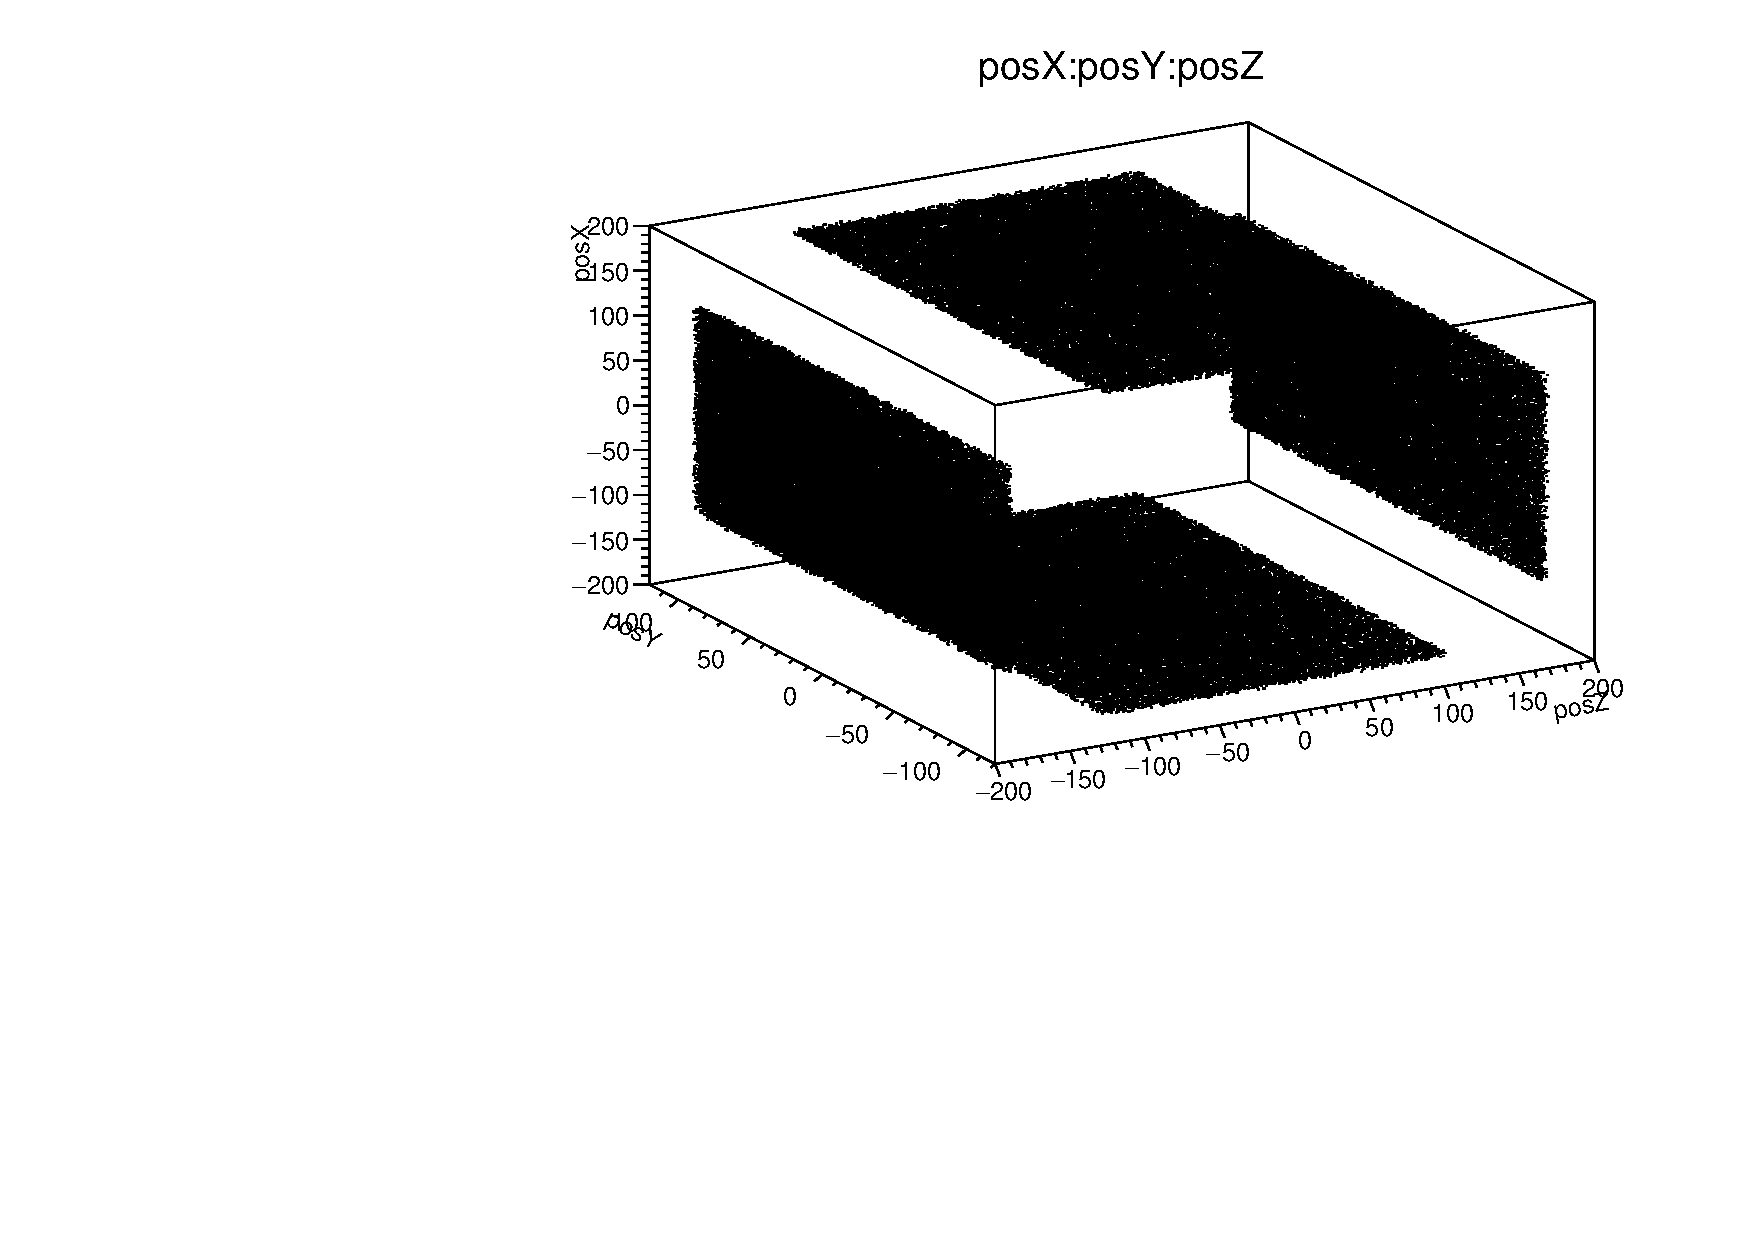
\includegraphics[scale=0.37]{figs/3Dhist.pdf}
\caption{Output of Draw command}
\label{fig:1Dhist}
\end{figure}
\clearpage

\subsection{Colors, markers, lines}
\subsubsection{Color}
It is possible to change the colors, line and marker styles and size.
To change the color one can use \verb|TTree ->SetMarkerColor(n_of_color)| or \verb|TTree ->SetLineColor(n_of_color)|. The \verb|n_of_color| can be chosen from table in Figure~\ref{fig:root_colors}, for more information check\\ \href{https://root.cern.ch/doc/v606/classTColor.html}{https://root.cern.ch/doc/v606/classTColor.html}  %\hypref{}{} 

\begin{figure}[h]
\centering
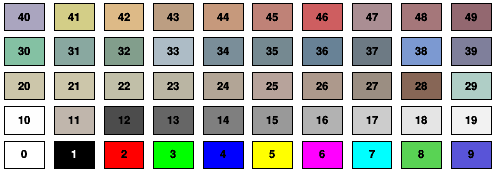
\includegraphics[scale=0.5]{figs/root_colors.png}
\caption{Basic ROOT colors used as a Draw() option. For more information check: \href{https://root.cern.ch/doc/v606/classTColor.html}{https://root.cern.ch/doc/v606/classTColor.html} }
\label{fig:root_colors}
\end{figure}

The example of usage is in the following command and in Figure~\ref{fig:1Dhist_color}:

root[4] \verb| Hits->SetLineColor(2) |

root[5] \verb| Hits->Draw("edep") | \\

or to change marker color one can do:\\

root[4] \verb| Hits->SetMarkerColor(2) |

root[5] \verb| Hits->Draw("edep") | \\
\begin{figure}[h]
\centering
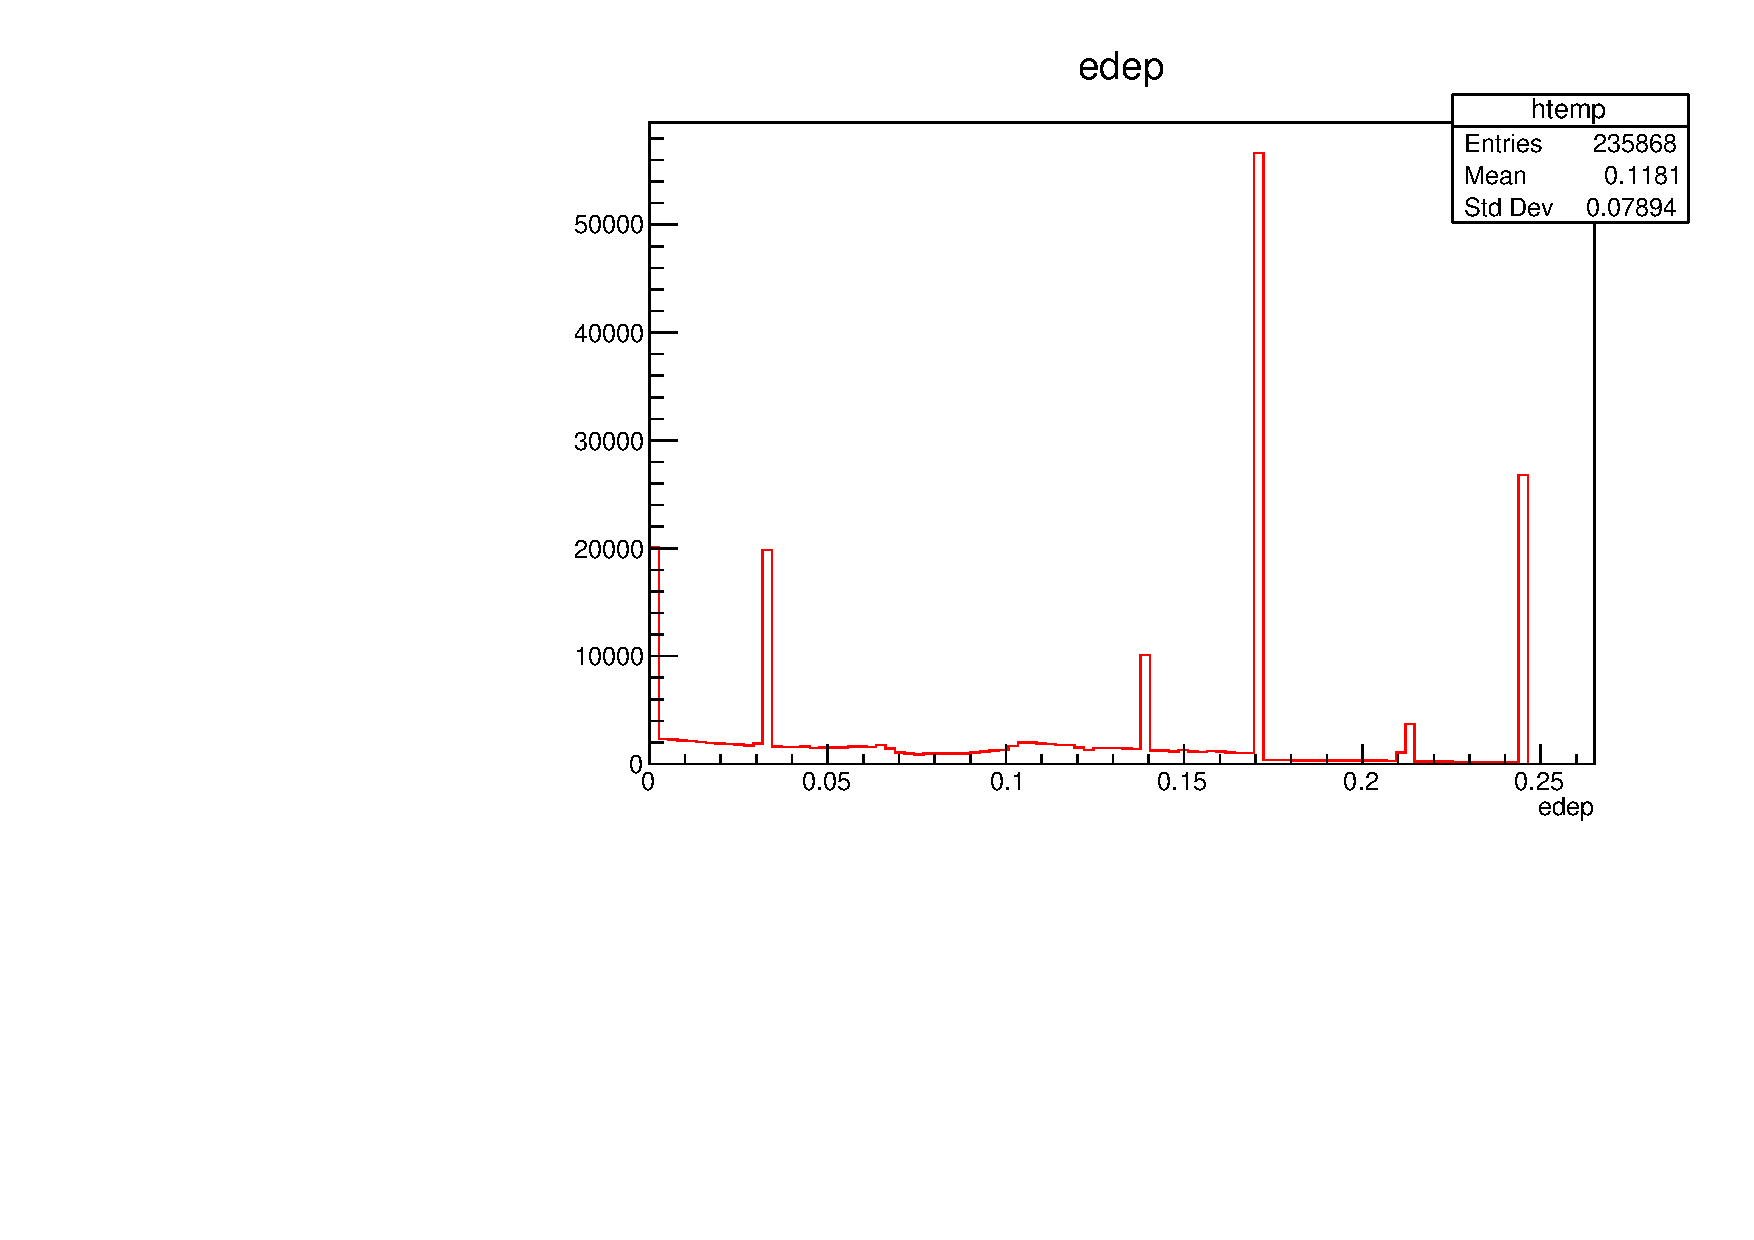
\includegraphics[scale=0.5]{figs/1Dhist_color.pdf}
\caption{Drawing of the 1D histogram with a color option}
\label{fig:1Dhist_color}
\end{figure}

\subsubsection{Size}
It is also possible to change size of lines with \verb|TTree ->SetLineWidth(size)|: \\

root[4] \verb| Hits->SetLineWidth(3) |

root[5] \verb| Hits->Draw("edep") | \\

\begin{figure}[h]
\centering
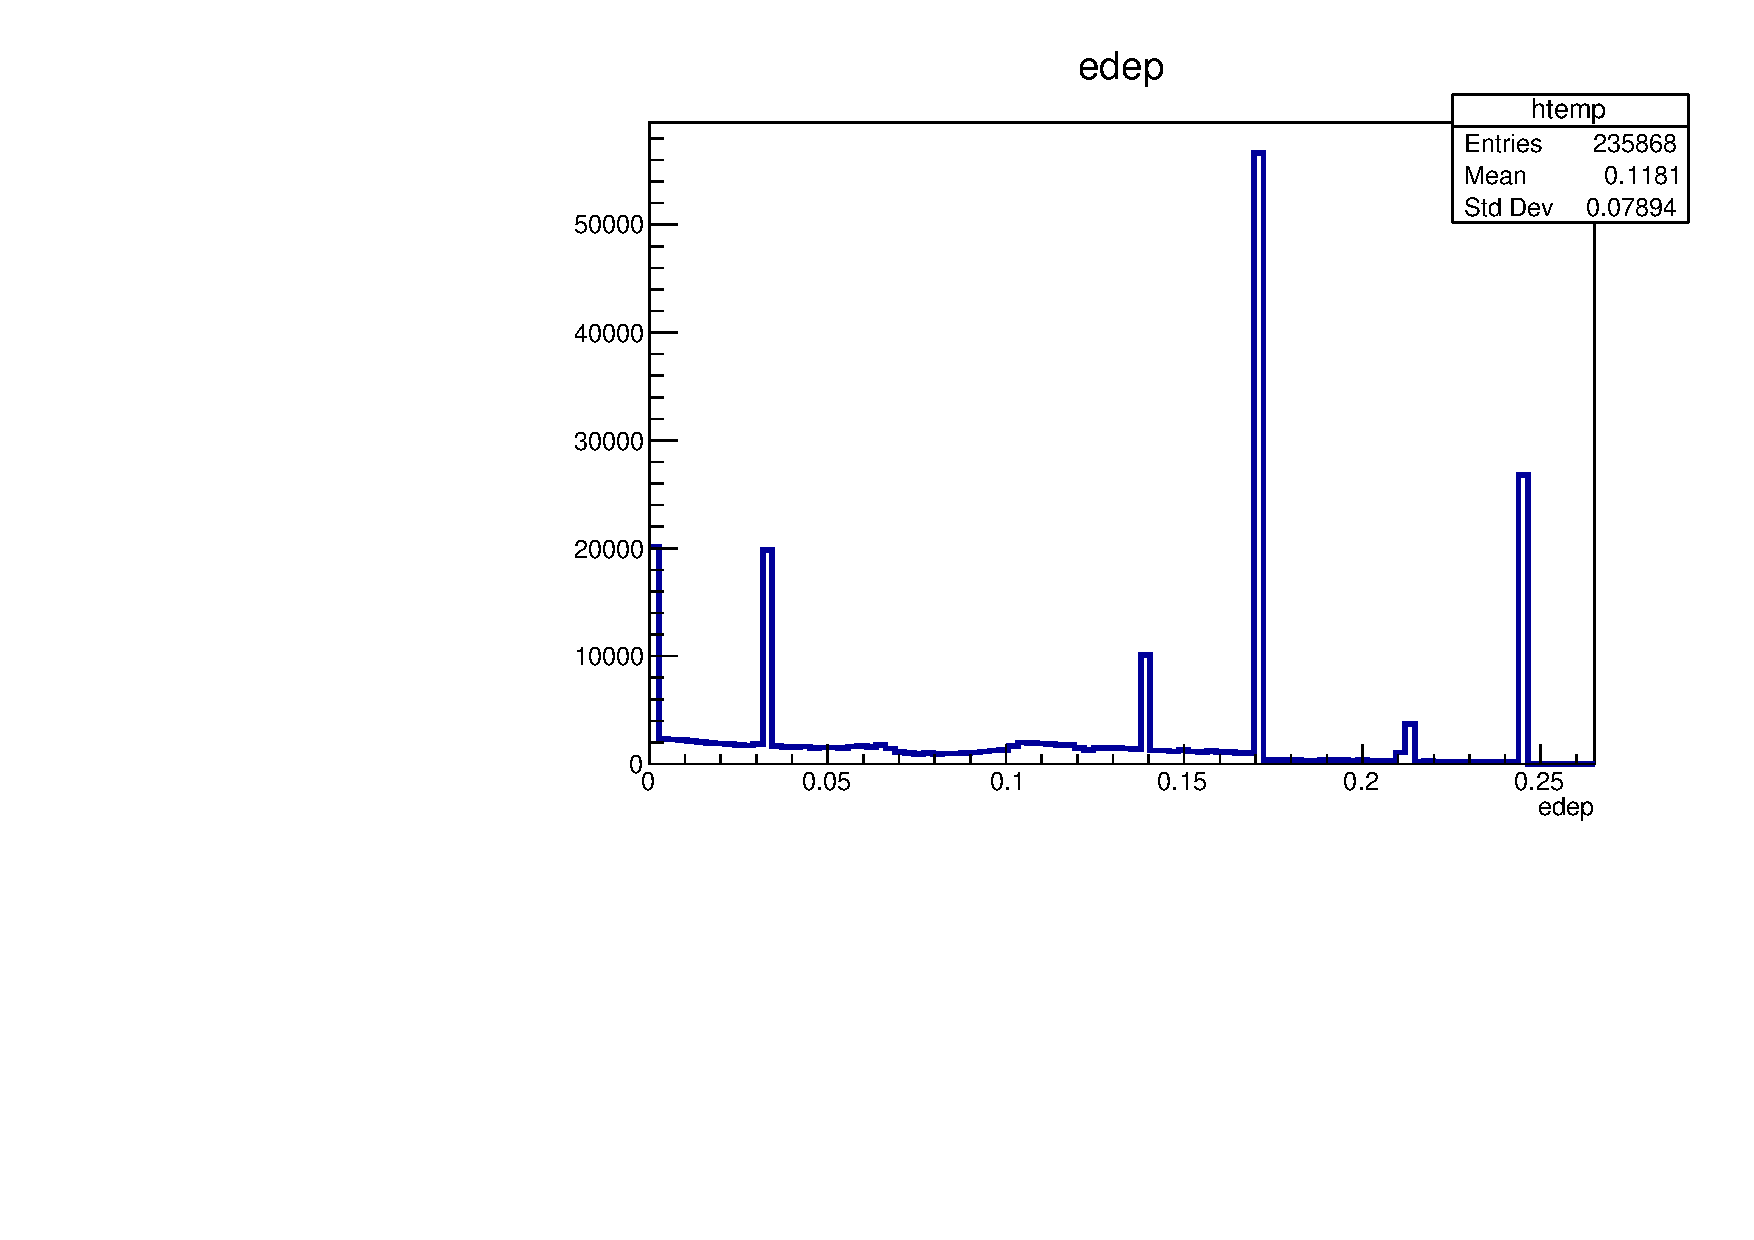
\includegraphics[scale=0.5]{figs/1Dhist_linewidth.pdf}
\caption{Drawing of the 1D histogram with a LineWidth option}
\label{fig:1Dhist_color}
\end{figure}

\subsubsection{Style}
It is also possible to change style of lines and markers with \verb|TTree ->SetLineStyle(n_of_style)| and  \verb|TTree ->SetLineStyle(n_of_style)|. The \verb|n_of_style| can be chosen from table in Figure~\ref{fig:root_linestyles} and in Figure~\ref{fig:root_markerstyles}, for more information check \\
\href{https://root.cern.ch/doc/v606/classTAttLine.html}{https://root.cern.ch/doc/v606/classTAttLine.html} and\\ \href{https://root.cern.ch/root/html534/TAttMarker.html}{https://root.cern.ch/root/html534/TAttMarker.html} \\

\begin{figure}[h]
\centering
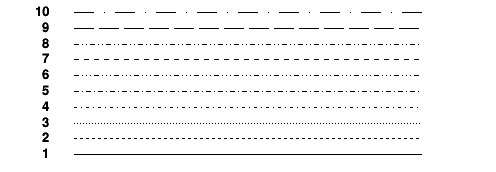
\includegraphics[scale=0.5]{figs/root_linestyles.png}
\caption{Basic ROOT line styles options. For more information check: \href{https://root.cern.ch/doc/v606/classTAttLine.html}{https://root.cern.ch/doc/v606/classTAttLine.html} }
\label{fig:root_linestyles}
\end{figure}

\begin{figure}[h]
\centering
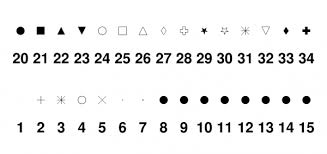
\includegraphics[scale=0.5]{figs/root_markerstyles.jpeg}
\caption{Basic ROOT marker styles options. For more information check: \href{https://root.cern.ch/root/html534/TAttMarker.html}{https://root.cern.ch/root/html534/TAttMarker.html}}
\label{fig:root_markerstyles}
\end{figure}

An example how to use these options is in the following and the results are illustrated in Figure~\ref{fig:1Dhist_linestyle} and in Figure~\ref{fig:2Dhist_markerstyle}:\\

root[4] \verb| Hits->SetLineStyle(4) |

root[5] \verb| Hits->Draw("edep") | \\

and \\

root[4] \verb| Hits->SetMarkerStyle(4) |

root[5] \verb| Hits->Draw("time:trackLength") | \\

\begin{figure}[h]
\centering
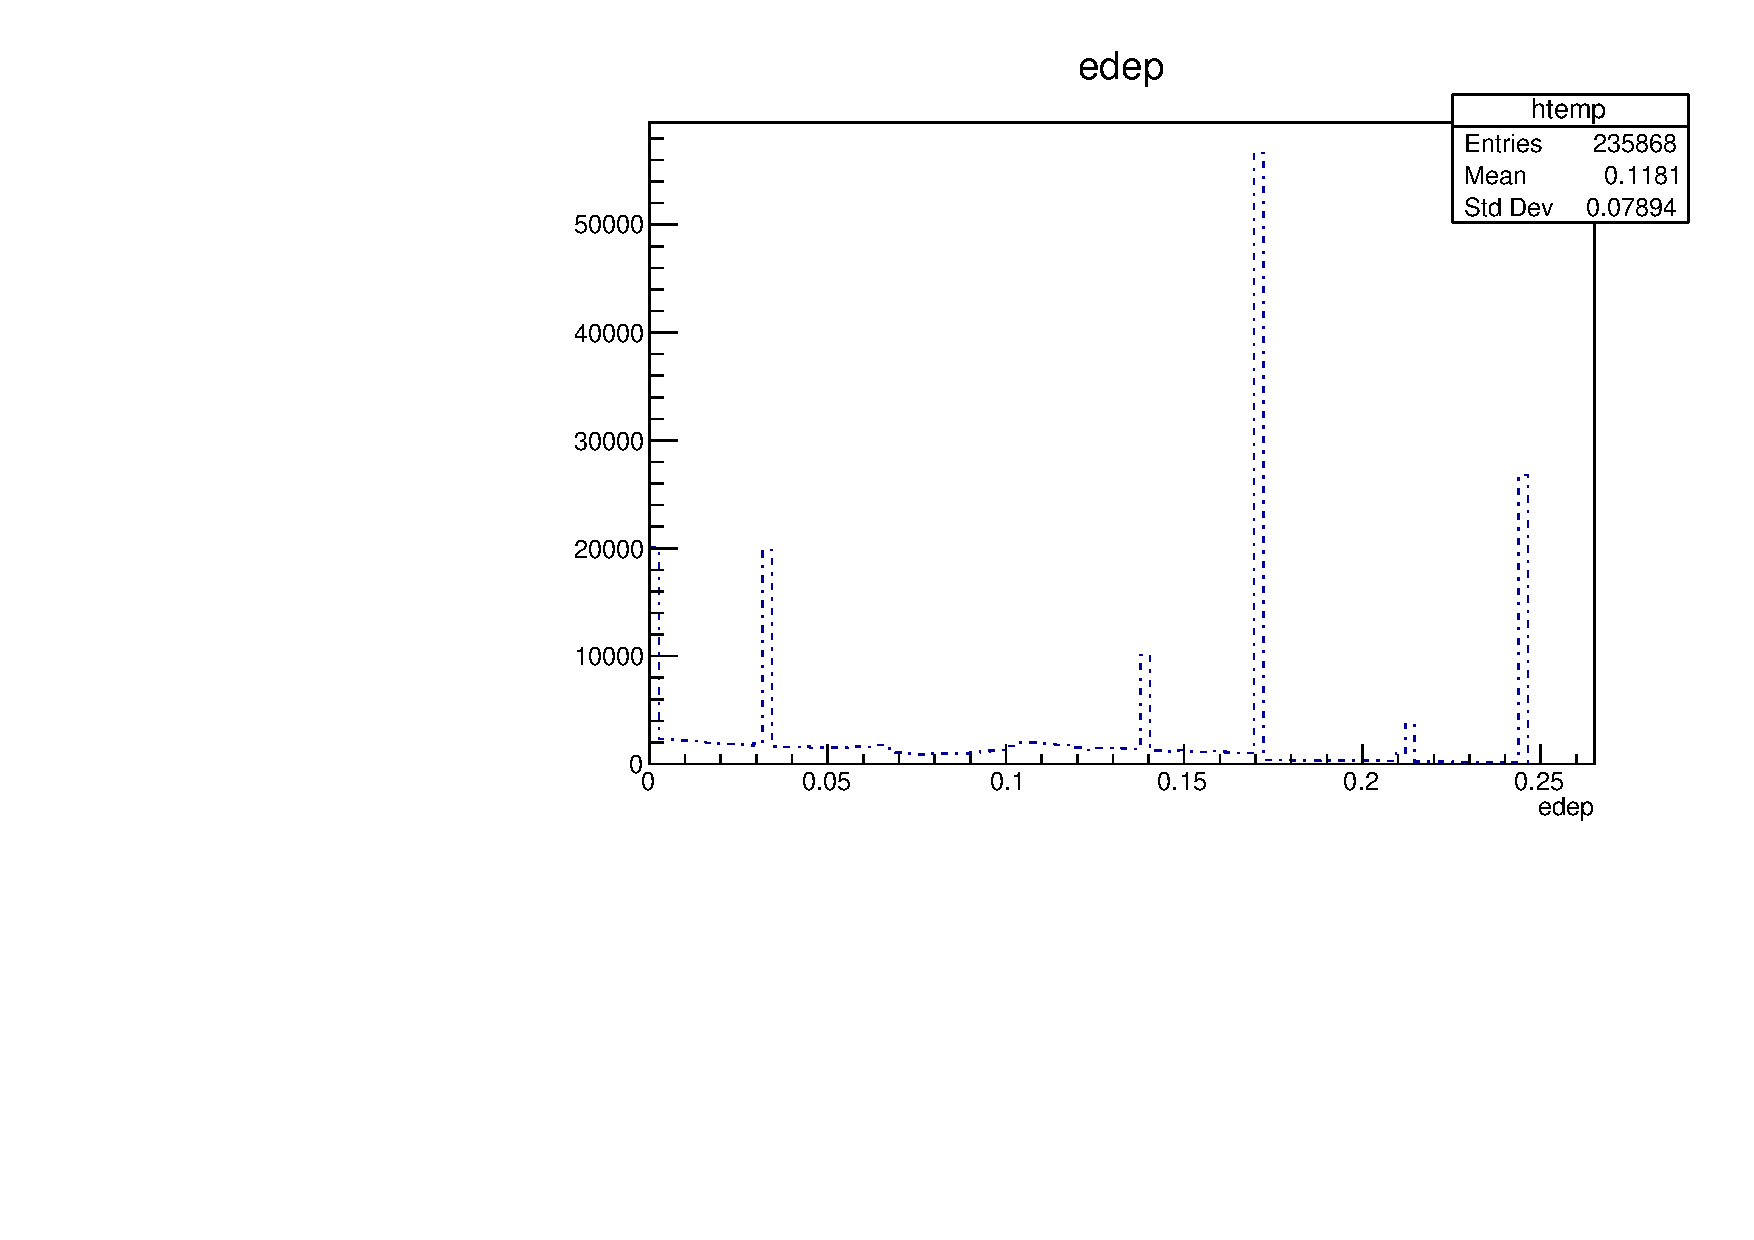
\includegraphics[scale=0.5]{figs/1Dhist_linestyle.pdf}
\caption{Drawing of the 1D histogram with a LineStyle option}
\label{fig:1Dhist_linestyle}
\end{figure}

\begin{figure}[h]
\centering
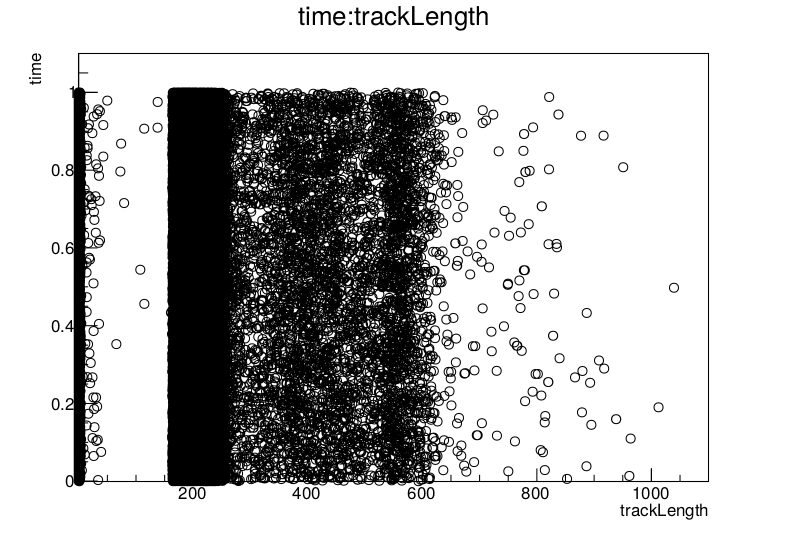
\includegraphics[scale=0.5]{figs/2Dhist_markerstyle.png}
\caption{Drawing of the 2D histogram with a MarkerStyle option}
\label{fig:2Dhist_markerstyle}
\end{figure}

\clearpage
\subsection{How to apply a simple selection}
It is also possible to apply a selection and after plot your variable. To do so one should use second option of the Draw() function: \verb|TTree ->Draw("name_of_the_branch","selection")|. The several examples of cuts are presented here and plot the effect of them on \verb|edep| variable:\\

root[4] \verb| Hits->Draw("edep","trackID==1") |

root[5] \verb| Hits->Draw("edep","posX>0.5") |

root[6] \verb| Hits->Draw("edep","localPosX>=0.5") |

root[7] \verb| Hits->Draw("edep","processName==\"phot\"") | (variable is a string)\\

Or even more complicated selections like: \\

root[8] \verb| Hits->Draw("edep","trackID==1 && posX>0.5") |

root[9] \verb| Hits->Draw("edep","trackID==1| $||$ \verb| posX>0.5") |\\

\subsection{How to rebin a histogram}
The default binning of 1D histogram in ROOT is 100 bins per X axis. It is possible to change and the simplest way is the following:\\
One has to defined a histogram with needed parameters:\\

root[1] \verb|TH1F* h = new TH1F("h","h",50,0,0.3) |\\

Here  we have a histogram with 50 bins in a range from 0 to 0.3.

Next step is to plot your histogram using the defined histogram "h" (Figure~\ref{fig:rebin}): \\

root[2] \verb| Hits->Draw("edep>>h","","") |

\begin{figure}[h]
\centering
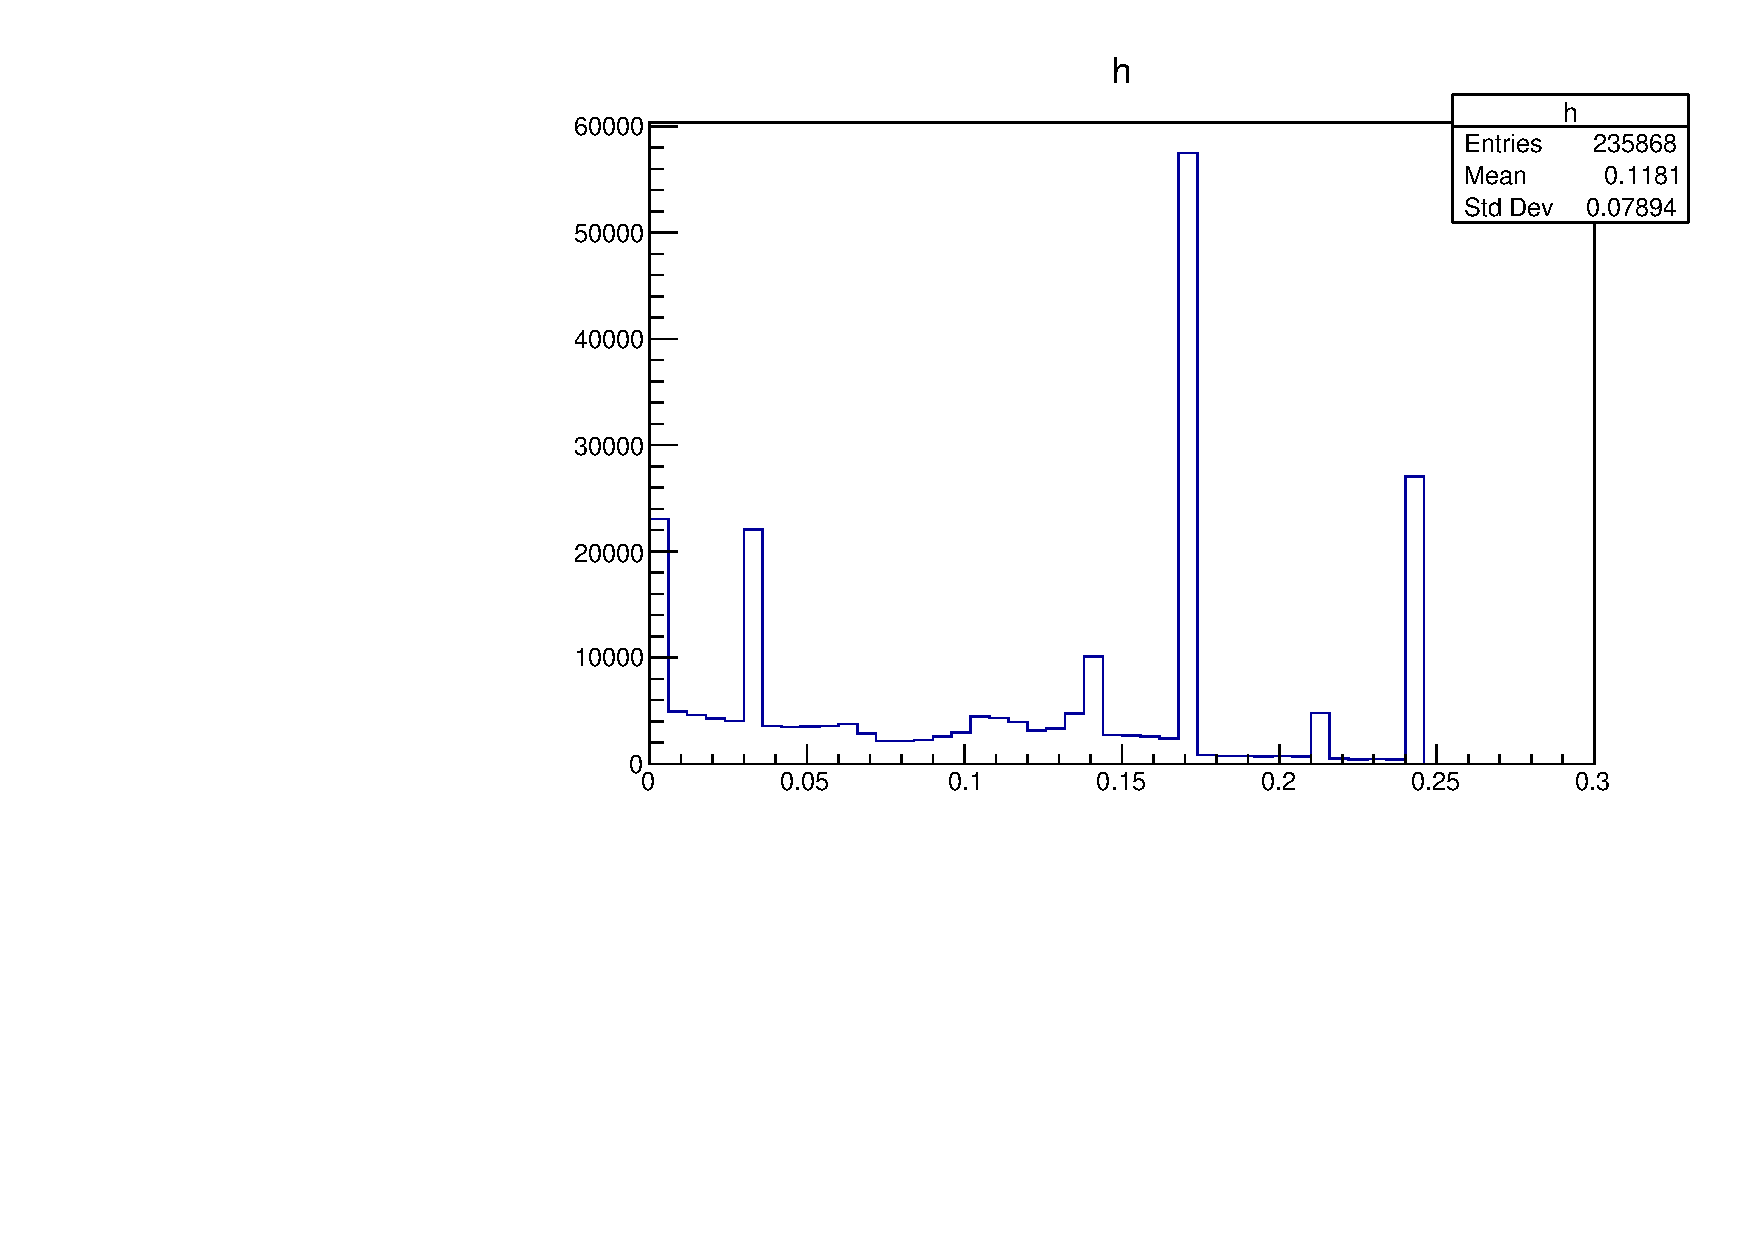
\includegraphics[scale=0.5]{figs/1Drebinning.pdf}
\caption{Drawing of rebinned 1D histogram}
\label{fig:rebin}
\end{figure}

\clearpage
\subsection{Superposition of two distributions}
 To superimpose two or more histograms one should write word "same" in the third option of the Draw() function: \verb|TTree ->Draw("name_of_the_branch","selection","same")|. For example, to obtain a histogram like in Figure~\ref{fig:1Dhist_cut} one can do: \\

root[4] \verb| Hits->Draw("edep","") |

root[5] \verb| Hits->SetLineColor(2)|

root[6] \verb| Hits->Draw("edep","processName==\"phot\"","same") |\\

\begin{figure}[h]
\centering
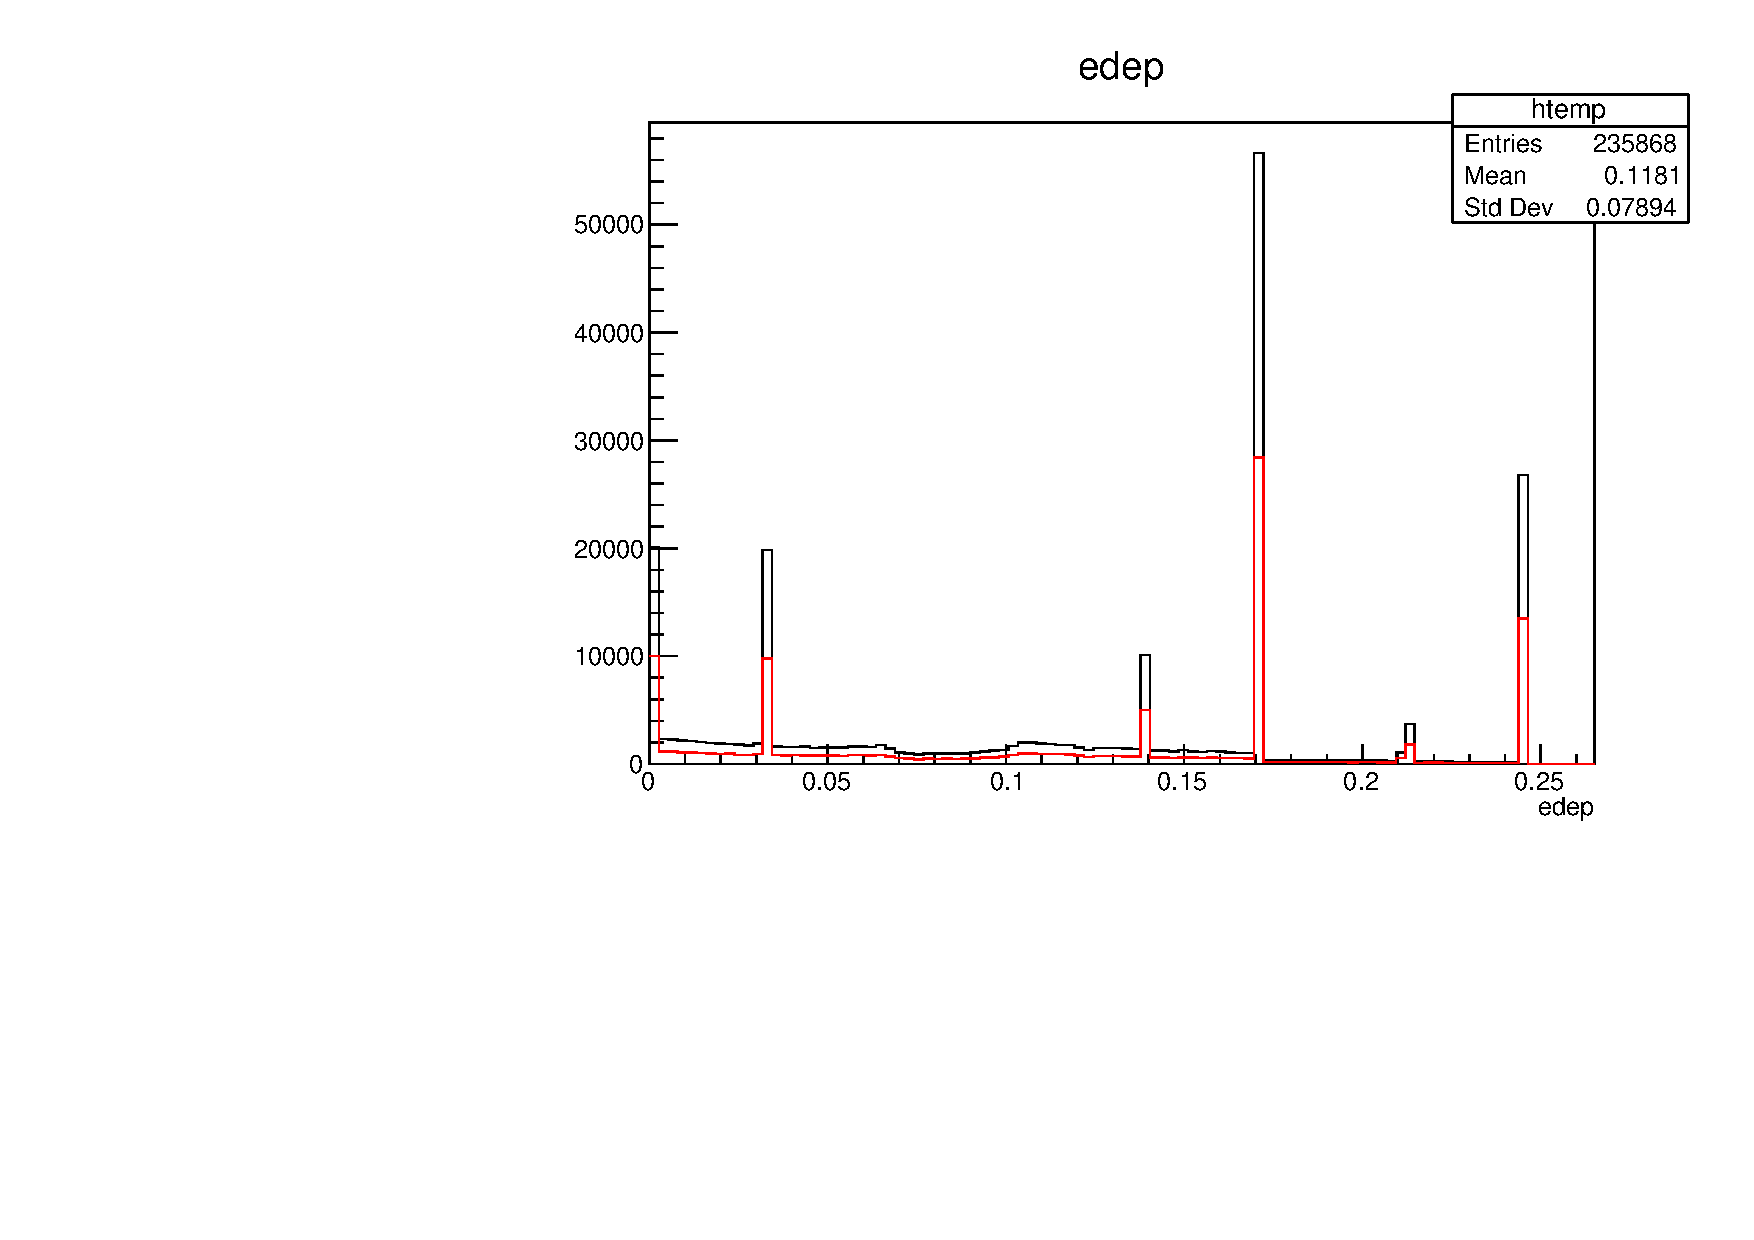
\includegraphics[scale=0.5]{figs/1Dhist_cut.pdf}
\caption{Drawing of two superposed the 1D histogram: one without any selection (black) and with a cut (red)}
\label{fig:1Dhist_cut}
\end{figure}

There is also a possibility to use \verb|"esame"| option for the fast comparison of two histograms. Actually, this option plot error bars (\verb|"e"| stands for that) but I would not recommend to rely on it and \textbf{calculate and plot your own error bars}. However, for a fast and easy superposition of two histograms without changing of line color it works perfectly (Figure~\ref{fig:1Dhist_esame}):\\

root[4] \verb| Singles->Draw("energy") |

root[5] \verb| Singles->Draw("energy","time<0.3","esame") |\\

\begin{figure}[h]
\centering
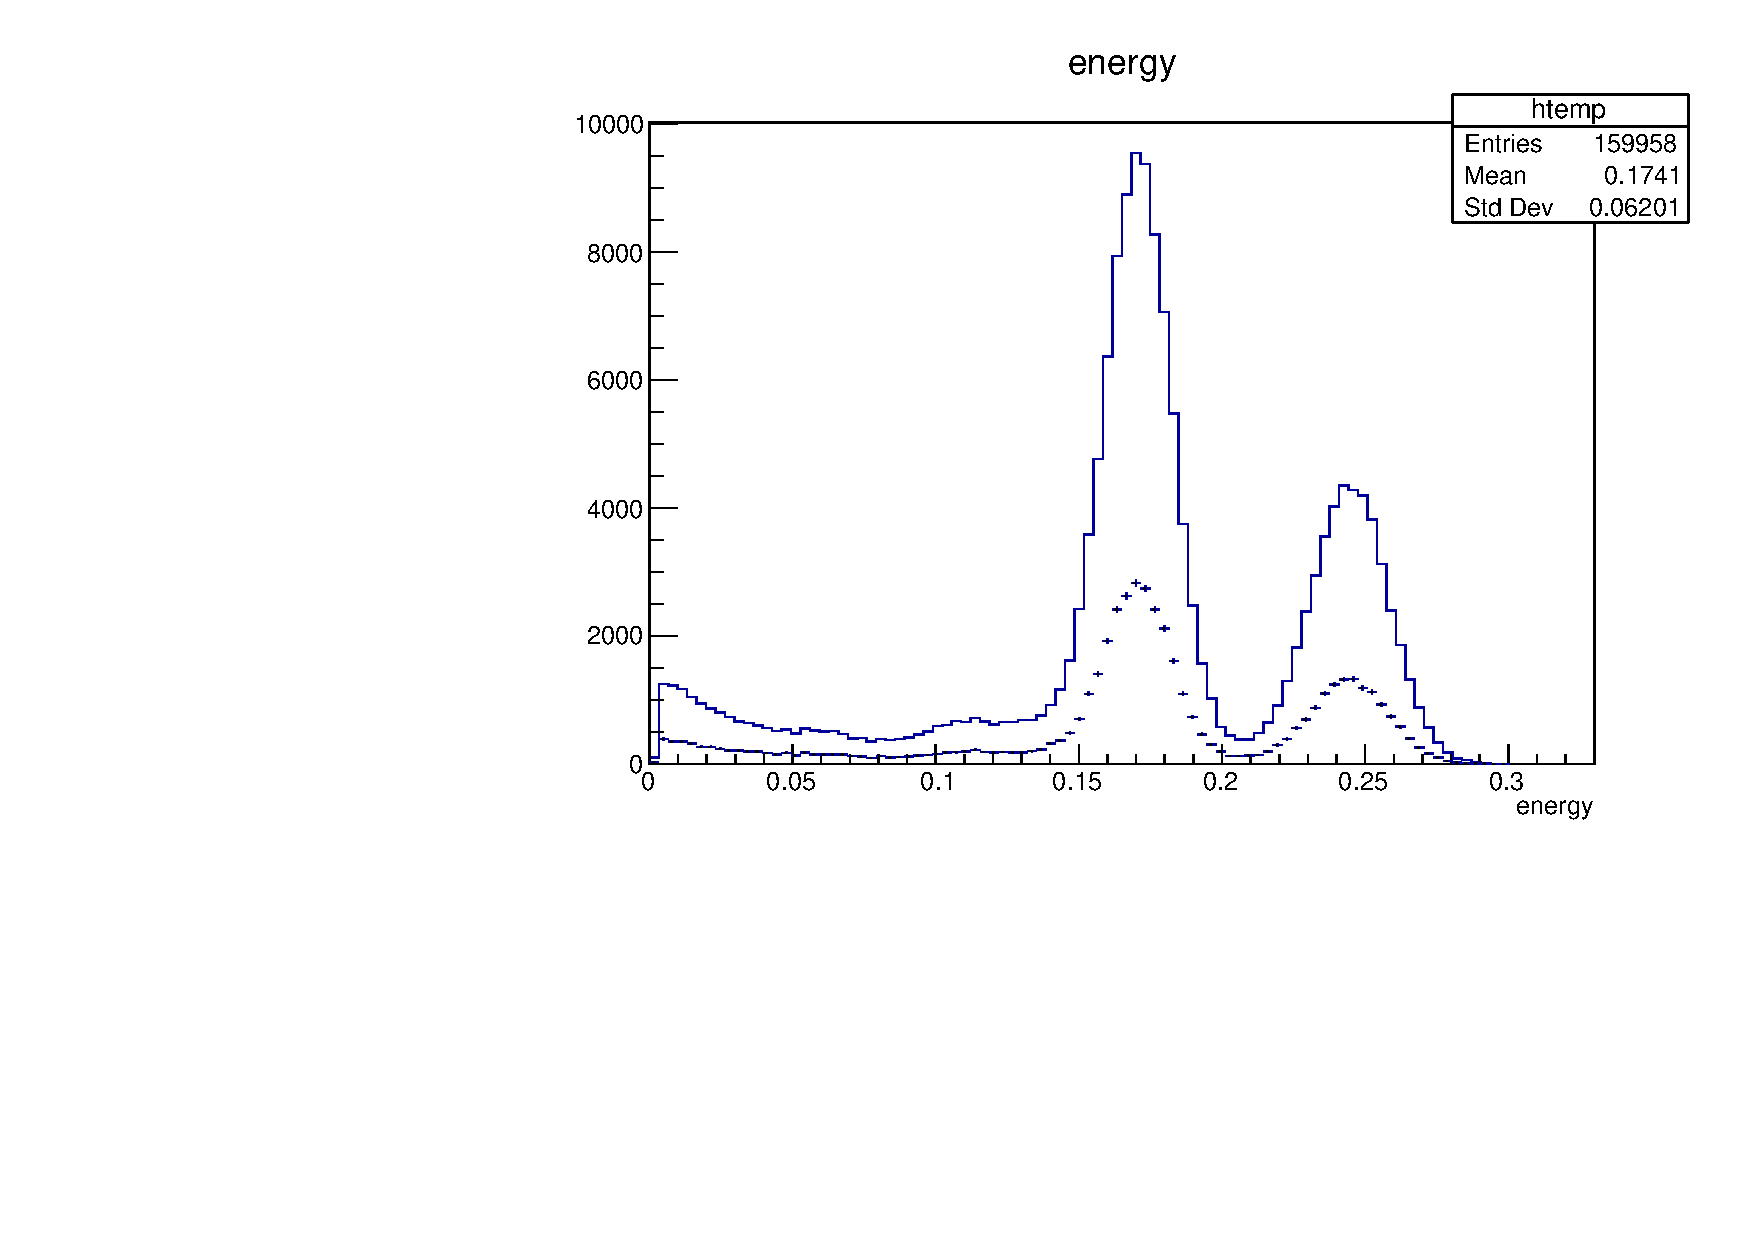
\includegraphics[scale=0.5]{figs/1Dhist_esame.pdf}
\caption{Drawing of two superposed the 1D histogram with "esame" option}
\label{fig:1Dhist_esame}
\end{figure}

\clearpage
\subsection{Superposition of two distributions from different ROOT files}
Sometimes it is useful to plot a superposition of two histograms from different ROOT files. In this case on start by opening the ROOT file 1:\\ 

\verb|> root -l YourOutputFile.root |\\

or by an equivalent command directly in ROOT:\\

root[0] \verb|  TFile *_file0 = TFile::Open("YourOutputFile.root");|\\

and drawing a histogram:\\

root[2] \verb| Singles->Draw("energy") | \\

The next step is to open the second file by: \\

root[3] \verb|  TFile *_file1 = TFile::Open("YourOutputFile1.root");|\\

and draw the new histogram with "same" or "esame" option:\\

root[4] \verb| Singles->Draw("energy","","esame") |\\


\subsection{Simple fitting}
It is possible to do a simple fit of your distribution. For this after drawing your histogram you need to go to the canvas window and select \verb| Tools --> Fit Panel |. You will have new window with a Fit Panel as presented in Figure~\ref{fig:FitPanel}. There you can choose your fitting function, fitting method, fitting range etc. In the following example, the fit is done by Gaussian function in the range [0.13;0.21]~MeV. The parameters of the fit is printed in the terminal window where you started ROOT and looks like following:
\verb| FCN=1259.74 FROM MIGRAD    STATUS=CONVERGED      75 CALLS      76 TOTAL|\\
\verb|                EDM=1.82902e-12    STRATEGY= 1      ERROR MATRIX ACCURATE| \\
\verb|   EXT PARAMETER                                   STEP         FIRST|   \\
\verb|   NO.   NAME      VALUE            ERROR          SIZE      DERIVATIVE |\\
\verb|    1  Constant     9.05059e+03   4.05523e+01   5.29487e-01  -2.23836e-09 |\\
\verb|    2  Mean         1.70049e-01   4.42797e-05   7.60710e-07  -4.18082e-02|\\
\verb|    3  Sigma        1.28126e-02   3.88904e-05   1.30065e-05  -8.44577e-04|\\

More about the fitting options can be found on ROOT web page.

\begin{figure}[h]
\centering
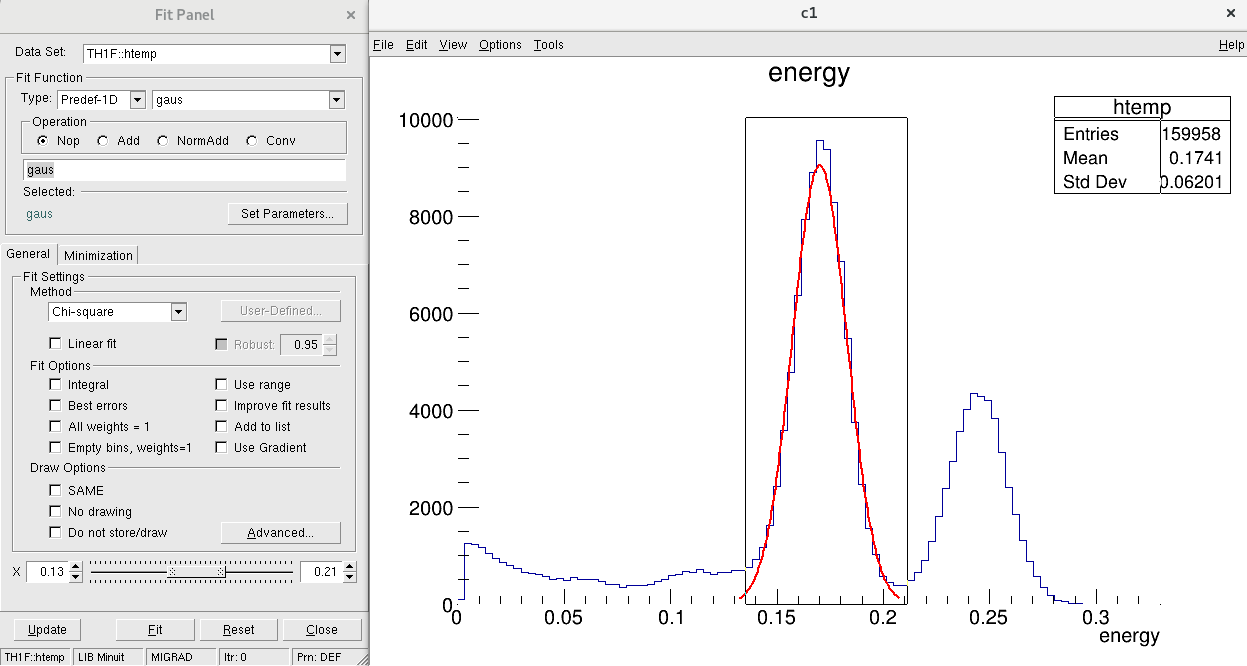
\includegraphics[scale=0.35]{figs/FitPanel.png}
\caption{Fit panel and an example of fitted histogram}
\label{fig:FitPanel}
\end{figure}


\section{Scan option}
Sometimes it is useful to printout the content of a branch, for example, in case when you want to study some anomalies. For this purpose one can use \verb|Scan()| function. It is similar to \verb|Draw()|, i.e. you also can apply cuts and plot several variables. For example, if one does: \\
root[4] \verb| Hits->Scan("edep:posX","time<0.1&&posY>0") |\\

the output will be something like this:\\
\verb|************************************|\\
\verb|*    Row   *      edep *      posX *|\\
\verb|************************************|\\
\verb|*        4 * 0.0198734 * 25.182537 *|\\
\verb|*        5 *         0 * 25.227350 *|\\
\verb|*       11 *         0 * -180.9978 *|\\
\verb|*       14 * 0.2450000 * 104.99372 *|\\
\verb|*       15 * 0.1710000 * -91.10610 *|\\
\verb|*       18 * 0.2199750 * 58.401462 *|\\
\verb|*       21 * 0.2450000 * -181.6459 *|\\
\verb|*       24 * 0.0803248 * 176.01010 *|\\
\verb|*       27 * 0.1520019 * -38.77223 *|\\
\verb|*       29 * 0.2450000 * 34.775840 *|\\
\verb|*       30 * 0.0811032 * -176.0955 *|\\
\verb|*       33 * 0.1103092 * -69.64908 *|\\
\verb|*       34 * 0.0957561 * -68.88422 *|\\
\verb|*       38 * 0.2450000 * 21.076614 *|\\
\verb|*       42 * 0.1710000 * -178.0622 *|\\
\verb|*       43 * 0.1710000 * -1.295397 *|\\
\verb|*       44 * 0.1387058 * 178.04272 *|\\
\verb|*       45 * 0.0322941 * 178.14222 *|\\
\verb|*       48 * 0.2450000 * -177.6772 *|\\
\verb|*       54 * 0.2450000 * -105.5232 *|\\
\verb|*       55 * 0.0675205 * -176.8821 *|\\
\verb|*       56 * 0.0562481 * 7.8245472 *|\\
\verb|*       57 * 0.1557220 * 7.5984726 *|\\
\verb|*       58 * 0.0330297 * 7.5733656 *|\\
\verb|*       60 * 0.1710000 * -47.08741 *|\\
\verb|Type <CR> to continue or q to quit ==>|\\
There are only first 25 lines in the output, one can press either "Enter" to continue or "q" to exit.

\clearpage
\section{Simplest script to draw with ROOT}
Sometimes it is useful to group the previous commands in a small script. Let's call it \verb|my_script.C|, in order to run it one can do: \\
 \verb|> root -l my_script.C |\\
 
The \verb|my_script.C| should contain something like this: \\
 \verb|{|\\
 \verb|  TFile *_file0 = TFile::Open("YourOutputFile.root");|\\
 \verb|  Singles->Draw("energy");|\\
 \verb|  Singles->Draw("energy","time<0.3","esame");|\\
 \verb|}|,\\
where you open file at the beginning and after you can copy you plotting commands.

\section{Example of script making beautiful plots}
I hear all the time a lot of complains that the ROOT plots are not beautiful.  Thus, in this section I propose you a template to start for your plots. To run the script one should do:\\
 \verb|> root -l my_script.C |\\

The name of the main function in \verb|my_script.C| must be the same as the name of your script file containing the following: \\
 \verb|void my_script() {| \\ 
 \verb|  //remove the stat from upper right corner|\\
 \verb|  gStyle->SetOptStat(0);|\\
 \verb|   //remove the title|\\
 \verb|   gStyle->SetOptTitle(0);|\\
 \verb|  //define fonts sizes|\\
 \verb|  gStyle->SetTextSize(0.06);|\\
 \verb|  gStyle->SetLabelSize(0.06,"x");|\\
 \verb|  gStyle->SetLabelSize(0.06,"y");|\\
 \verb|  gStyle->SetLabelSize(0.06,"z");|\\
 \verb|  gStyle->SetTitleSize(0.06,"x");|\\
 \verb|  gStyle->SetTitleSize(0.05,"y");|\\
 \verb|  gStyle->SetTitleSize(0.06,"z");|\\
 \verb|  //define number of divisions on any axis, here is done only for "Y"|\\
\verb|  gStyle->SetNdivisions(505,"y");|\\
\verb|  gStyle->SetLineWidth(3);|\\

\verb|  //define your ROOT file name|\\ 
\verb|      TString filename = "YourOutputFile.root";|\\
 
\verb|  // open the file|\\  
\verb|      TFile *f = TFile::Open(filename);|\\
\verb|    // get the TTree|\\  
\verb|      TTree *Tree = (TTree*)f->Get("Singles");|\\

\verb|  // define the variable(s) of interest, type of variable must be respected|\\    
\verb|      Float_t energy;|\\

\verb|  // define the branch(s) of interest|\\    
\verb|      TBranch *benergy;|\\

\verb|  // Set branch address|\\ 
\verb|      Tree->SetBranchAddress( "energy", &energy, &benergy);|\\
   
\verb|  // Get number of events in the TTree|\\
\verb|      const int n=(const int)Tree->GetEntries();|\\

\verb|  // Define a histogram with 100 bins, on x from 0 to 0.3|\\
\verb|    TH1F* h = new TH1F("h","h",100,0,0.3); |\\

\verb|  // Loop over events |\\	   
\verb|    for(int i=0;i<n;i++)|\\
\verb|     {|\\
\verb|      //get event i|\\
\verb|      Tree->GetEntry(i);|\\
\verb|      benergy->GetEntry(i);|\\
\verb|      //print out the values |\\    
\verb|      cout<<i<<" "<<energy<<endl;|\\
\verb|	     //fill histogram|\\
\verb|      h->Fill(energy);|\\	
\verb|      }|\\	

\verb|	//Define canvas|\\
\verb|    TCanvas *can = new TCanvas("can","can",600,800);|\\

\verb|	//Define paramters of the canvas|\\
\verb|	    can->SetFillColor(0);|\\
\verb|	    can->SetBorderMode(0);|\\
\verb|	    can->SetBorderSize(3);|\\
\verb|	    can->SetBottomMargin(0.14);|\\
\verb|	    can->SetLeftMargin(0.16);|\\
\verb|	    can->SetFrameBorderMode(0);|\\
\verb|	    can->SetFrameLineWidth(3);|\\
\verb|	    can->SetFrameBorderMode(0);|\\

\verb|//Define parameters of the histogram|\\
\verb|  h->SetLineWidth(2);|\\
\verb|  h->SetLineColor(2);|\\
\verb|  h->GetXaxis()->SetTitle("Energy, MeV");|\\
\verb|  h->GetYaxis()->SetTitleOffset(1.6);|\\ 
\verb|  h->GetYaxis()->SetTitle("Arbitrary units"); |\\  
\verb|	//Draw histogram|\\
\verb|  h->Draw();|\\
\verb|  //Save cancas as .pdf|\\
\verb|  can->SaveAs("energy.pdf");|\\
\verb|}|

This script could also be found
\href{https://github.com/kochebina/ROOT_manual_for_Gate_users/tree/master/Materials}{here}.  

The output result is shown in Figure~\ref{fig:energy}.

\begin{figure}[h]
\centering
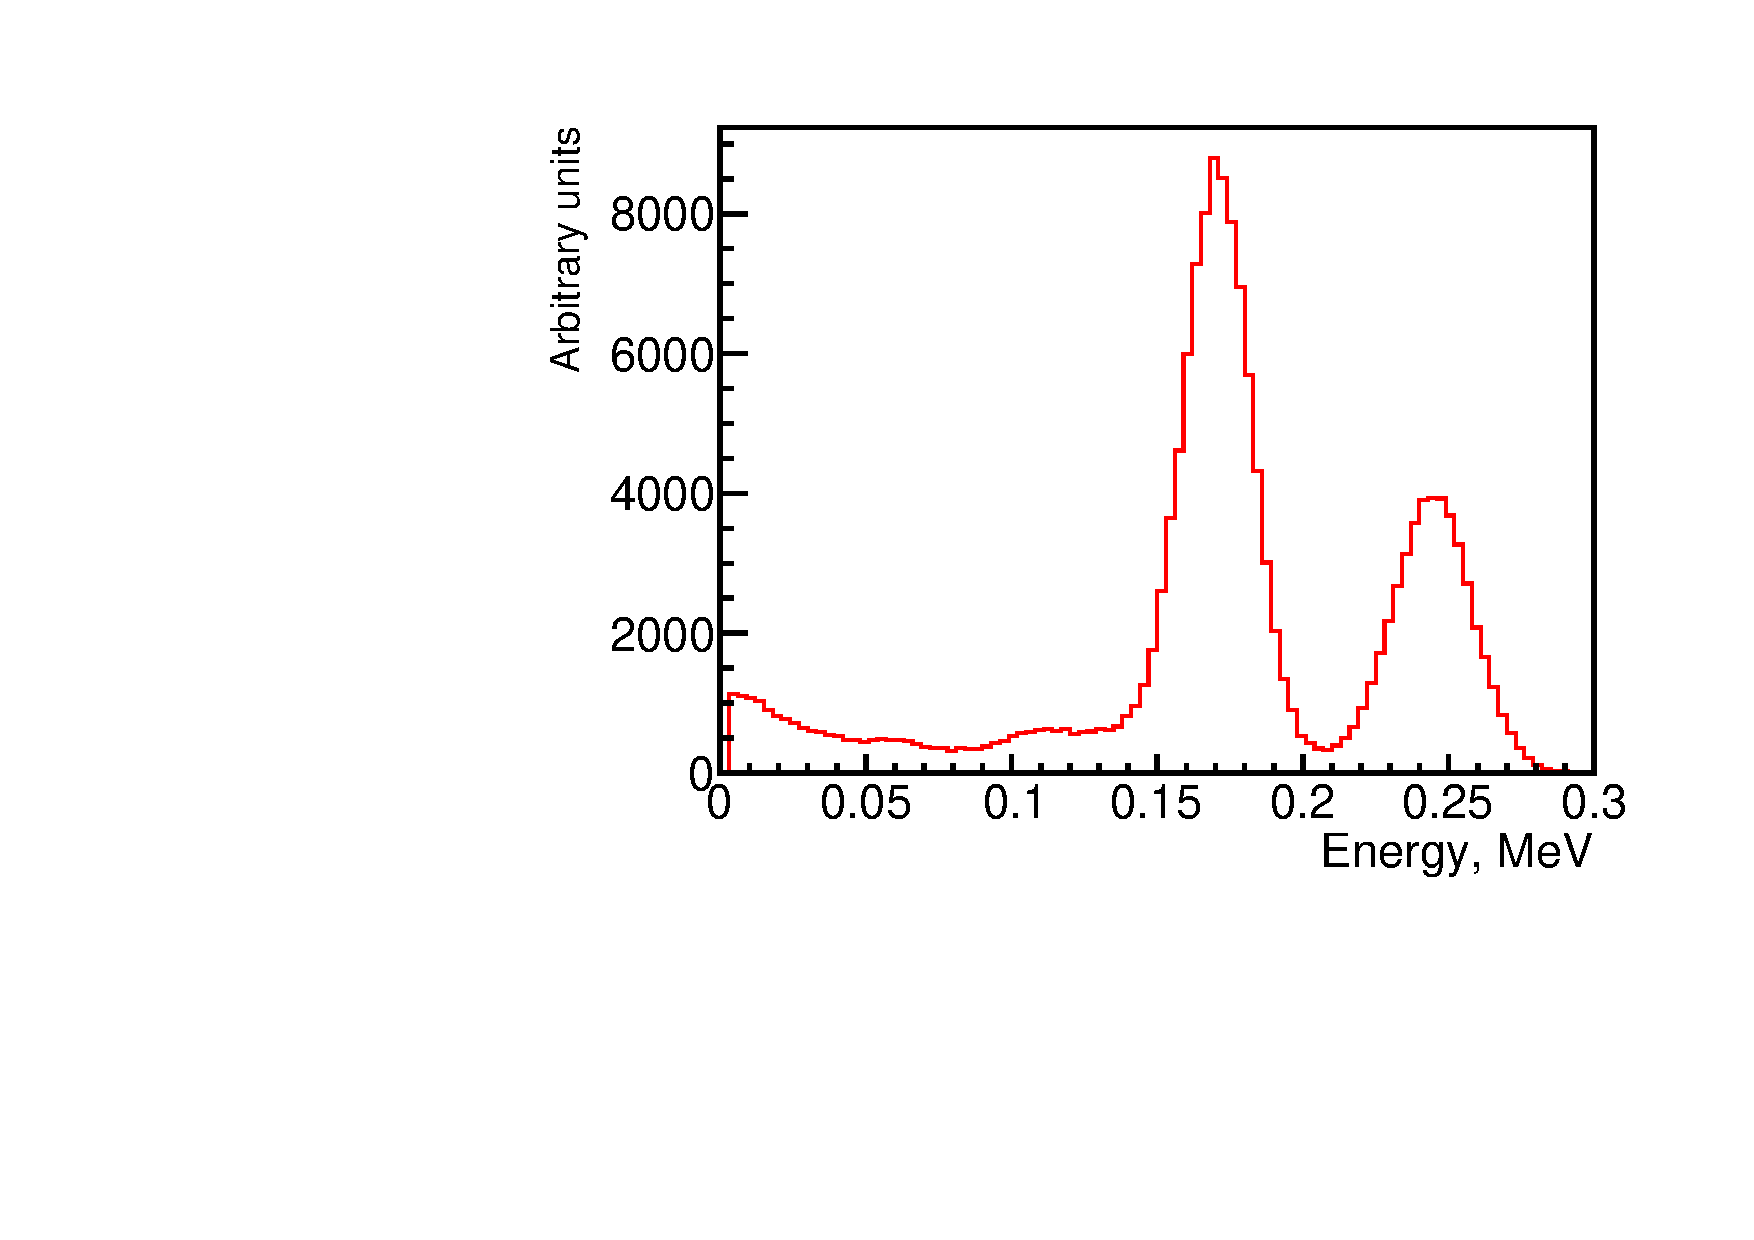
\includegraphics[scale=0.6]{figs/energy.pdf}
\caption{The output of the example of script making beautiful plots.}
\label{fig:energy}
\end{figure}


\clearpage
\section{Adding a new variable to your TTree*}
In this section I will just add a link to the script that indicates how to add a new variable. It is a script that adds a shift on energy which is different for each of four detection heads.   



%\apendix




%\bibliographystyle{plain}
%\bibliography{biblio}



\end{document}